\documentclass{beamer}
\usepackage{amsmath}
\usepackage[english]{babel} %set language; note: after changing this, you need to delete all auxiliary files to recompile
\usepackage[utf8]{inputenc} %define file encoding; latin1 is the other often used option
\usepackage{csquotes} % provides context sensitive quotation facilities
\usepackage{graphicx} %allows for inserting figures
\usepackage{booktabs} % for table formatting without vertical lines
\usepackage{textcomp} % allow for example using the Euro sign with \texteuro
\usepackage{stackengine}
\usepackage{wasysym}
\usepackage{tikzsymbols}
\usepackage{textcomp}
\newcommand{\bubblethis}[2]{
        \tikz[remember picture,baseline]{\node[anchor=base,inner sep=0,outer sep=0]%
        (#1) {\underline{#1}};\node[overlay,cloud callout,callout relative pointer={(0.2cm,-0.7cm)},%
        aspect=2.5,fill=yellow!90] at ($(#1.north)+(-0.5cm,1.6cm)$) {#2};}%
    }%
\tikzset{face/.style={shape=circle,minimum size=4ex,shading=radial,outer sep=0pt,
        inner color=white!50!yellow,outer color= yellow!70!orange}}
%% Some commands to make the code easier
\newcommand{\emoticon}[1][]{%
  \node[face,#1] (emoticon) {};
  %% The eyes are fixed.
  \draw[fill=white] (-1ex,0ex) ..controls (-0.5ex,0.2ex)and(0.5ex,0.2ex)..
        (1ex,0.0ex) ..controls ( 1.5ex,1.5ex)and( 0.2ex,1.7ex)..
        (0ex,0.4ex) ..controls (-0.2ex,1.7ex)and(-1.5ex,1.5ex)..
        (-1ex,0ex)--cycle;}
\newcommand{\pupils}{
  %% standard pupils
  \fill[shift={(0.5ex,0.5ex)},rotate=80] 
       (0,0) ellipse (0.3ex and 0.15ex);
  \fill[shift={(-0.5ex,0.5ex)},rotate=100] 
       (0,0) ellipse (0.3ex and 0.15ex);}

\newcommand{\emoticonname}[1]{
  \node[below=1ex of emoticon,font=\footnotesize,
        minimum width=4cm]{#1};}
\usepackage{scalerel}
\usetikzlibrary{positioning}
\usepackage{xcolor,amssymb}
\newcommand\dangersignb[1][2ex]{%
  \scaleto{\stackengine{0.3pt}{\scalebox{1.1}[.9]{%
  \color{red}$\blacktriangle$}}{\tiny\bfseries !}{O}{c}{F}{F}{L}}{#1}%
}
\newcommand\dangersignw[1][2ex]{%
  \scaleto{\stackengine{0.3pt}{\scalebox{1.1}[.9]{%
  \color{red}$\blacktriangle$}}{\color{white}\tiny\bfseries !}{O}{c}{F}{F}{L}}{#1}%
}
\usepackage{fontawesome} % Social Icons
\usepackage{epstopdf} % allow embedding eps-figures
\usepackage{tikz} % allows drawing figures
\usepackage{amsmath,amssymb,amsthm} %advanced math facilities
\usepackage{lmodern} %uses font that support italic and bold at the same time
\usepackage{hyperref}
\usepackage{tikz}
\hypersetup{
    colorlinks=true,
    linkcolor=blue,
    filecolor=magenta,      
    urlcolor=blue,
}
\usepackage{tcolorbox}
%add citation management using BibLaTeX
\usepackage[citestyle=authoryear-comp, %define style for citations
    bibstyle=authoryear-comp, %define style for bibliography
    maxbibnames=10, %maximum number of authors displayed in bibliography
    minbibnames=1, %minimum number of authors displayed in bibliography
    maxcitenames=3, %maximum number of authors displayed in citations before using et al.
    minnames=1, %maximum number of authors displayed in citations before using et al.
    datezeros=false, % do not print dates with leading zeros
    date=long, %use long formats for dates
    isbn=false,% show no ISBNs in bibliography (applies only if not a mandatory field)
    url=false,% show no urls in bibliography (applies only if not a mandatory field)
    doi=false, % show no dois in bibliography (applies only if not a mandatory field)
    eprint=false, %show no eprint-field in bibliography (applies only if not a mandatory field)
    backend=biber %use biber as the backend; backend=bibtex is less powerful, but easier to install
    ]{biblatex}
\addbibresource{../mybibfile.bib} %define bib-file located one folder higher


\usefonttheme[onlymath]{serif} %set math font to serif ones

\definecolor{beamerblue}{rgb}{0.2,0.2,0.7} %define beamerblue color for later use

%%% defines highlight command to set text blue
\newcommand{\highlight}[1]{{\color{blue}{#1}}}


%%%%%%% commands defining backup slides so that frame numbering is correct

\newcommand{\backupbegin}{
   \newcounter{framenumberappendix}
   \setcounter{framenumberappendix}{\value{framenumber}}
}
\newcommand{\backupend}{
   \addtocounter{framenumberappendix}{-\value{framenumber}}
   \addtocounter{framenumber}{\value{framenumberappendix}}
}

%%%% end of defining backup slides

%Specify figure caption, see also http://tex.stackexchange.com/questions/155738/caption-package-not-working-with-beamer
\setbeamertemplate{caption}{\insertcaption} %redefines caption to remove label "Figure".
%\setbeamerfont{caption}{size=\scriptsize,shape=\itshape,series=\bfseries} %sets figure  caption bold and italic and makes it smaller


\usetheme{Boadilla}

%set options of hyperref package
\hypersetup{
    bookmarksnumbered=true, %put section numbers in bookmarks
    naturalnames=true, %use LATEX-computed names for links
    citebordercolor={1 1 1}, %color of border around cites, here: white, i.e. invisible
    linkbordercolor={1 1 1}, %color of border around links, here: white, i.e. invisible
    colorlinks=true, %color links
    anchorcolor=black, %set color of anchors
    linkcolor=beamerblue, %set link color to beamer blue
    citecolor=blue, %set cite color to beamer blue
    pdfpagemode=UseThumbs, %set default mode of PDF display
    breaklinks=true, %break long links
    pdfstartpage=1 %start at first page
    }


% --------------------
% Overall information
% --------------------
\title[Principios de Economía]{Principios de Economía}
\date{}
\author[Ertola y Sturzenegger]{Gabriela Ertola y Federico Sturzenegger }
\vspace{0.4cm}
\institute[]{Universidad de San Andrés \\
2022} 


\begin{document}

\begin{frame}
\frametitle{Principios de Economía
\centering
\\ \vspace{12mm} Teoría del Productor}
\centering
 \\ \vspace{12mm} %5 de agosto, 2021 \vspace{5mm} \\ 

\includegraphics[scale=0.25]{Figures/logoUDESA.jpg} 
\end{frame}

\begin{frame}
\frametitle{ El comportamiento de la firma}
\begin{itemize}
    \item ¿Cuál es el objetivo de las empresas? \vspace{2mm} \\
    \hspace{18mm} ¡¡¡GANAR DINERO!!! \vspace{2mm} \\
    \item El éxito de una empresa – y su capacidad de crecer – dependen en parte de las decisiones que toman las empresas
    \begin{itemize}
        \item Pero estas decisiones dependen: \\
        - de las características del mercado, y \\
        - de los costos de producción
        \item También las políticas gubernamentales pueden afectar la división de los excedentes entre las empresas y los clientes
    \end{itemize}    
\end{itemize}    
\end{frame}

\begin{frame}
\frametitle{Restricciones y decisiones}
\begin{itemize}
    \item La firma se enfrenta a dos grandes restricciones:
        \begin{itemize}
        \item Las características del mercado \\
        - ¿Qué es lo que los consumidores están dispuestos a comprar? \\
        - ¿Cómo se comportan las otras empresas?
        \item Sus capacidades tecnológicas \\
        - Las características de su función de producción dada por sus costos de producción
        \end{itemize}
    \item Tomando en cuenta estas restricciones, la empresa toma decisiones \\
    \begin{itemize}
        \item Sobre el precio al que ofrece sus productos...
        \item ... y la cantidad de este producto que genera
    \end{itemize}
\end{itemize} 
\end{frame}

\begin{frame}
\frametitle{¿Que información necesita la firma para decidir qué precio cobrar?}
\begin{itemize}
    \item Para decidir qué precio cobrar, una empresa necesita información sobre la demanda
    \begin{itemize}
        \item ¿Qué es la demanda? \\
    La demanda es cuánto están dispuestos a pagar los consumidores potenciales por su producto
    \end{itemize}
    \item Recuerden como estimamos la demanda de pizza de Eco I... ¡con una encuesta sobre la disposición a pagar!

\end{itemize}
\end{frame}

\begin{frame}
\frametitle{El problema de la firma}
\begin{itemize}
    \item Una vez que conocemos la demanda... ¿cómo se elige cuánto producir y el precio que cobrar?
    \vspace{2mm}
    \item El problema principal de la empresa es el de la maximización del beneficio
    \vspace{2mm}     \begin{itemize}
        \item ¿Qué es el beneficio? \vspace{2mm} \\ 
        Beneficio = Ingresos totales – Costos totales
        \vspace{2mm}
        \item ¿Qué es el ingreso total? 
        \vspace{2mm} \\ 
        El valor de la producción al precio ofrecido (p·q)
        \vspace{2mm}
        \item ¿Qué es el costo total?
        \vspace{2mm} \\ 
        Los costos por unidad, por la cantidad de unidades producidas (c·q)
    \end{itemize} 
\end{itemize} 
\end{frame}

\begin{frame}
\frametitle{Vamos a ser maestros pizzeros}
\centering

\includegraphics[scale=0.6]{Figures/Tema_06.12_maestrospizzeros.jpg}
\end{frame}

\begin{frame}
\frametitle{Pensando en los costos}
\begin{itemize}
    \item Costos explícitos
    \begin{itemize}
        \item Harina, levadura, sal, agua, etc.
        \item Alquiler del negocio (podríamos ser los dueños pero en ese caso...)
        \item Salario de los empleados 
        \item Servicios que hay que pagar (agua, luz, gas, etc.)
    \end{itemize}
    \item Costos implícitos
    \begin{itemize}
        \item El salario que perdemos por la actividad alternativa
        \item El costo del capital invertido (que podría ser utilizado en otra actividad económica)
    \end{itemize}
\end{itemize}
\end{frame}

\begin{frame}
\frametitle{Ganancia económica versus ganancia contable}
\centering
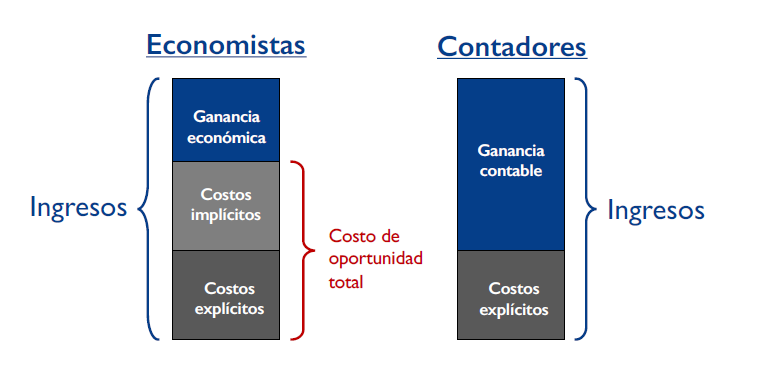
\includegraphics[scale=0.6]{Figures/Tema_06.13_beneficioeconomicovscontable.png}
\end{frame}

\begin{frame}
\frametitle{ En el corto plazo...}
\centering
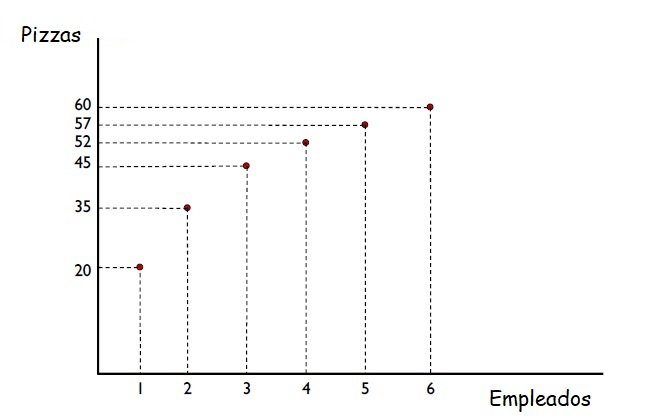
\includegraphics[scale=0.6]{Figures/Tema_06.14_funciondeproduccionmedialunas.jpg}
\end{frame}

\begin{frame}
\frametitle{Función de producción de pizzas}
\centering
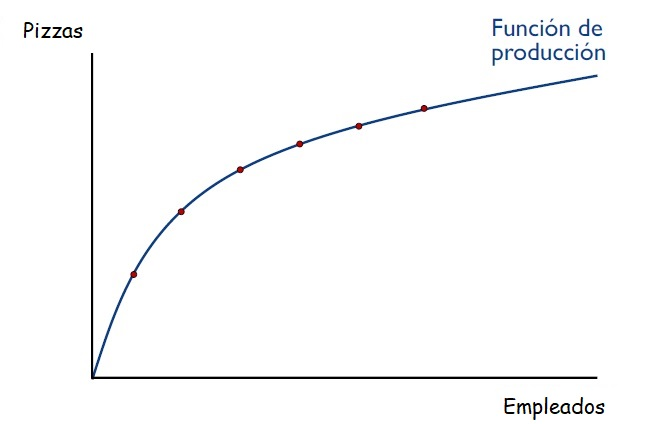
\includegraphics[scale=0.6]{Figures/Tema_06.15.jpg}
\end{frame}

\begin{frame}
\frametitle{ Contratando a un empleado adicional}
\centering
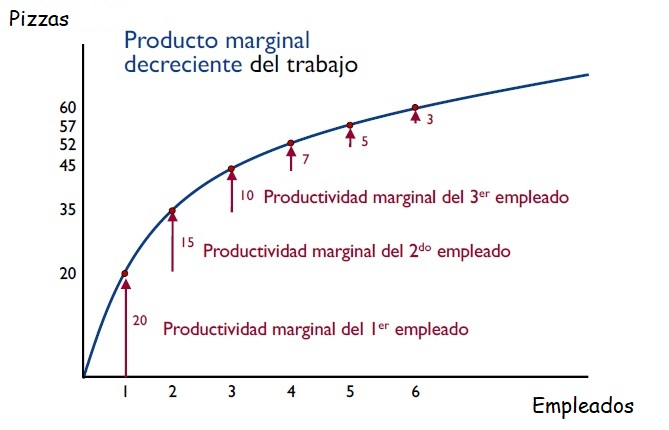
\includegraphics[scale=0.6]{Figures/Tema_06.16.jpg}
\end{frame}


\begin{frame}
\frametitle{Por un lado los costos fijos...}
\centering
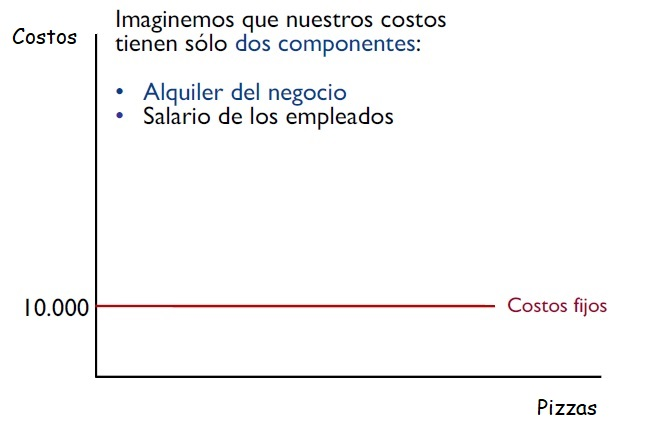
\includegraphics[scale=0.6]{Figures/Tema_06.17.jpg}
\end{frame}

\begin{frame}
\frametitle{ Por otro lado los costos variables}
\centering
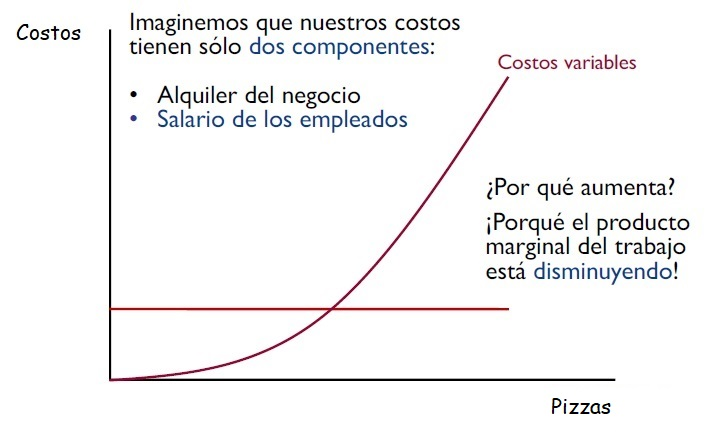
\includegraphics[scale=0.6]{Figures/Tema_06.18.jpg}
\end{frame}

\begin{frame}
\frametitle{ Los costos totales}
\centering
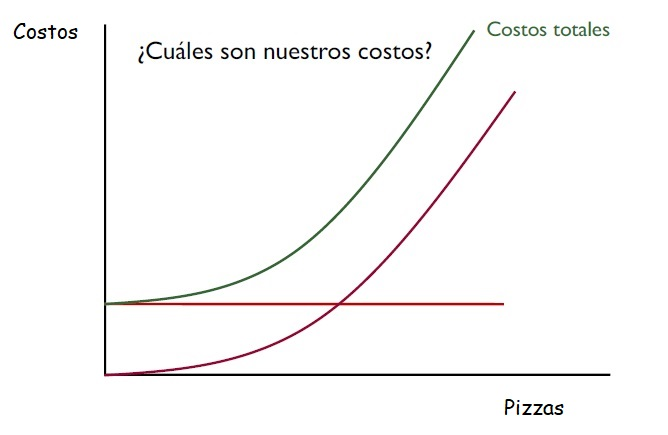
\includegraphics[scale=0.6]{Figures/Tema_06.19.jpg}
\end{frame}

\begin{frame}
\frametitle{ Los costos de hacer pizzas}
\begin{itemize}
    \item Se observan dos tipos de costos: 
        \begin{itemize}
        \item Los costos fijos
        \item Los costos variables
        \end{itemize}
    \vspace{2mm}
    \item Para evaluar la cantidad de pizzas que queremos producir nos vamos a hacer dos preguntas:
        \begin{itemize}
        \item ¿Cuánto cuesta en promedio una pizza?
        \item ¿Cuánto cuesta hacer una pizza adicional?
        \end{itemize}
\end{itemize}
\end{frame}

\begin{frame}
\frametitle{ Los costos medios y marginales}
\begin{itemize}
    \item El costo medio es el costo promedio por unidad producida
    \begin{itemize}
        \item Gráficamente es la pendiente del rayo que sale desde el origen a un punto dado de la función de costo \\
        - En el ejemplo, disminuye al principio pero luego aumentan 
    \end{itemize}
    \item El costo marginal mide el efecto sobre el costo total al producir una unidad adicional
    \begin{itemize}
        \item Gráficamente, es la pendiente de la función de costo en un punto dado \\
        - En el ejemplo, los costos marginales aumentan a medida que aumenta la producción
    \end{itemize}
\end{itemize}
\end{frame}

\begin{frame}
\frametitle{ ¿Cómo construir los costos medios?}
\centering
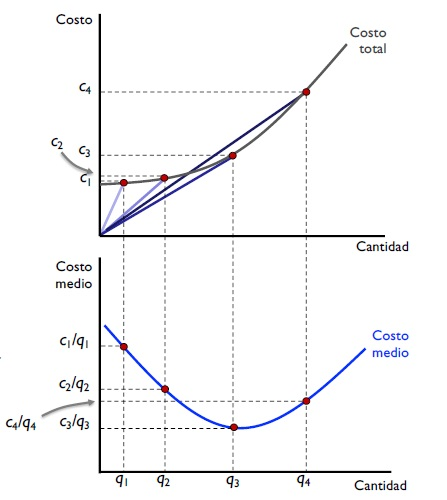
\includegraphics[scale=0.6]{Figures/Tema_06.21_funciondeproduccionmedialunas7.jpg}
\end{frame}

\begin{frame}
\frametitle{ ¿Cómo construir el costo marginal?}
\centering
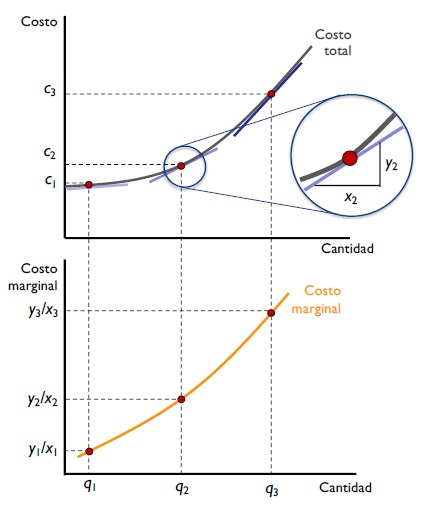
\includegraphics[scale=0.6]{Figures/Tema_06.26_costos5.jpg}
\end{frame}

\begin{frame}
\frametitle{ Graficando costo medio y marginal en el mismo gráfico}
\centering
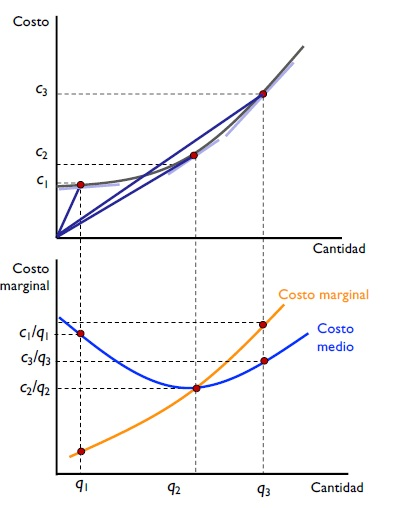
\includegraphics[scale=0.5]{Figures/Tema_06.27_costos6.jpg}
\end{frame}

\begin{frame}
\frametitle{ Los costos del negocio}
\centering
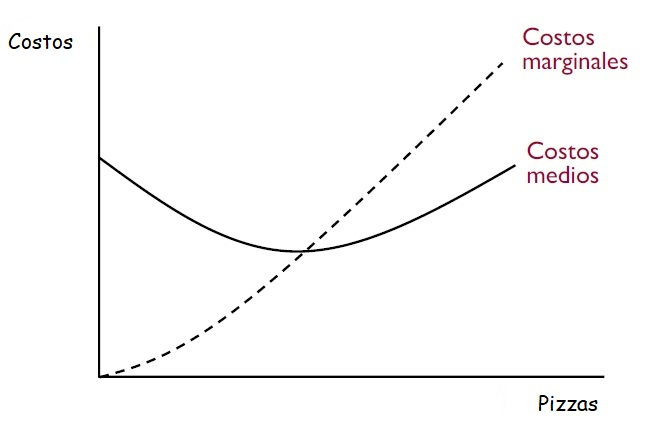
\includegraphics[scale=0.6]{Figures/Tema_06.20.jpg}
\end{frame}

\begin{frame}
\frametitle{ A largo plazo podemos crecer}
\begin{itemize}
    \item Los costos de una empresa dependen de su escala y el tipo de tecnología de producción
    \item Empresas grandes pueden ser más rentables que las pequeñas debido diversas ventajas:
    \begin{itemize}
        \item Ventajas tecnológicas \\
        - Producción a gran escala usa menos insumos
        \item Ventajas de costos \\
        - Por ejemplo, empresas grandes, con mayor poder de negociación, pueden comprar recursos en términos más favorables
        \item Ventajas de demanda \\
        - Por ejemplo, efectos de red (valor de la producción aumenta con el número de usuarios)
    \end{itemize}
\end{itemize}
\end{frame}

\begin{frame}
\frametitle{ Rendimientos a escala}
\begin{itemize}
    \item ¿Qué sucede con la producción cuando aumentamos la cantidad de insumos productivos en la misma proporción?
    \begin{itemize}
        \item La producción aumenta pero... ¿cómo aumenta?
    \end{itemize}
    \item Si la producción aumenta mas que proporcionalmente, entonces la función de producción exhibe rendimientos crecientes a escala (Economías de escala o costos decrecientes a escala)
\end{itemize}
\end{frame}

\begin{frame}
\frametitle{ Rendimientos a escala}
\begin{itemize}
    \item Si la producción aumenta proporcionalmente, entonces la función de producción exhibe rendimientos constantes a escala (Costos constantes a escala)
    \item Si la producción aumenta menos que proporcionalmente, entonces la función de producción exhibe rendimientos decrecientes a escala (Deseconomías de escala o costos crecicientes a escala)
\end{itemize}
\end{frame}

\begin{frame}
\frametitle{ Costos en el largo plazo}
\centering
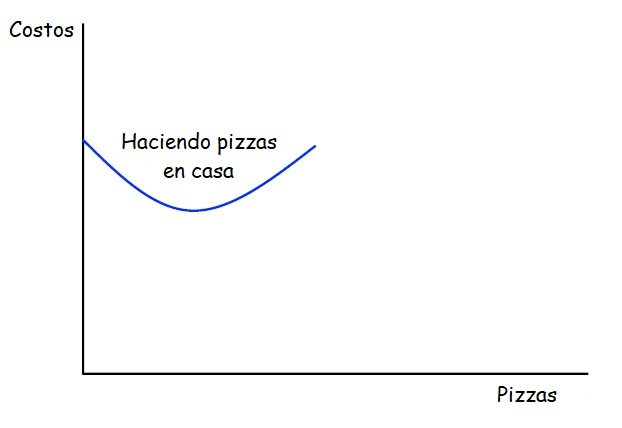
\includegraphics[scale=0.6]{Figures/Tema_06.24.jpg}
\end{frame}

\begin{frame}
\frametitle{ Costos en el largo plazo}
\centering
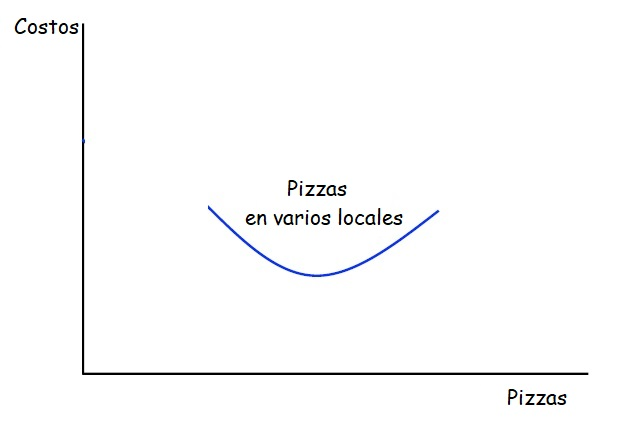
\includegraphics[scale=0.6]{Figures/Tema_06.25.jpg}
\end{frame}

\begin{frame}
\frametitle{ Costos en el largo plazo}
\centering
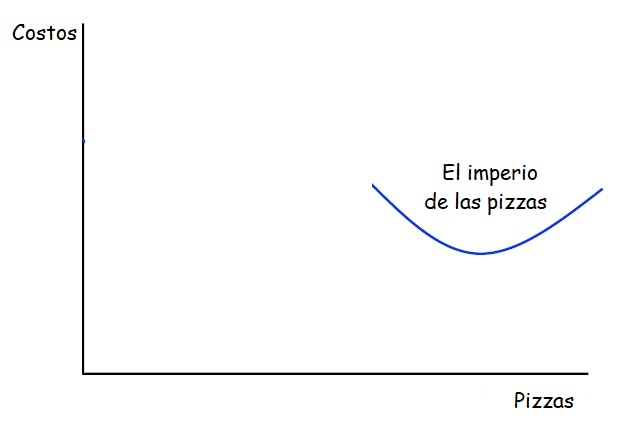
\includegraphics[scale=0.6]{Figures/Tema_06.26.jpg}
\end{frame}

\begin{frame}
\frametitle{ Costos en el largo plazo}
\centering
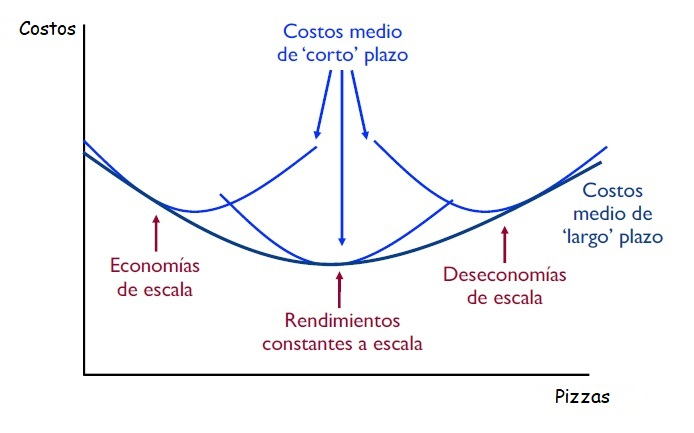
\includegraphics[scale=0.6]{Figures/Tema_06.25_costos4.jpg}
\end{frame}

\begin{frame}
\frametitle{ Margen de beneficio}
\begin{itemize}
    \item Por un momento, supongamos que el precio de la pizza es p
        \item ¿Me conviene producir una pizza adicional?     
    \begin{itemize}
        \item Si uno aumenta una unidad de producto, recibe p
        \item Pero al mismo tiempo sus costos se incrementan en Cmg
        \item Entonces, el beneficio extra que se recibe es p – CMg
        \end{itemize}
    \item La diferencia entre el precio (p) y el costo marginal (CMg) se denomina margen de beneficio
\end{itemize}
\end{frame}

\begin{frame}
\frametitle{ Conclusiones con un P fijo}
\begin{itemize}
    \item ¿Me conviene producir una pizza adicional?
        \begin{itemize}
        \item Si el margen de beneficios es positivo entonces SI, conviene producir una pizza adicional
        \item Pero si el margen de beneficios es negativo entonces NO conviene producir una pizza adicional
        \end{itemize} \\ \vspace{2mm}
    \item ¿Qué significa que el margen de beneficios sea igual 0?
\end{itemize}
\end{frame}

\begin{frame}
\frametitle{ Vamos a ver que pasa con diferentes precios....}
\begin{itemize}
\centering
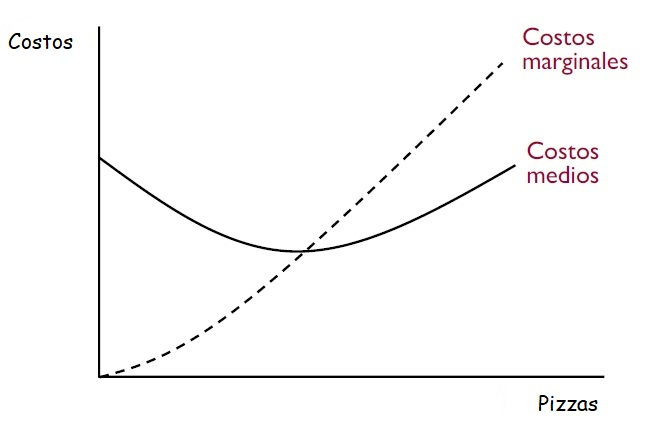
\includegraphics[scale=0.6]{Figures/Tema_06.20.jpg}
\end{itemize}
\end{frame}

\begin{frame}
\frametitle{ La curva de oferta de la empresa}
\centering
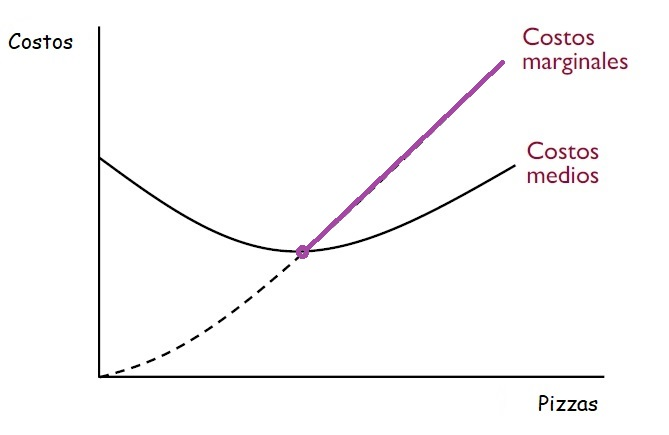
\includegraphics[scale=0.6]{Figures/Tema_06.28.jpg}
\end{frame}

\begin{frame}
\frametitle{ La curva de oferta del mercado de pizzas}
\centering
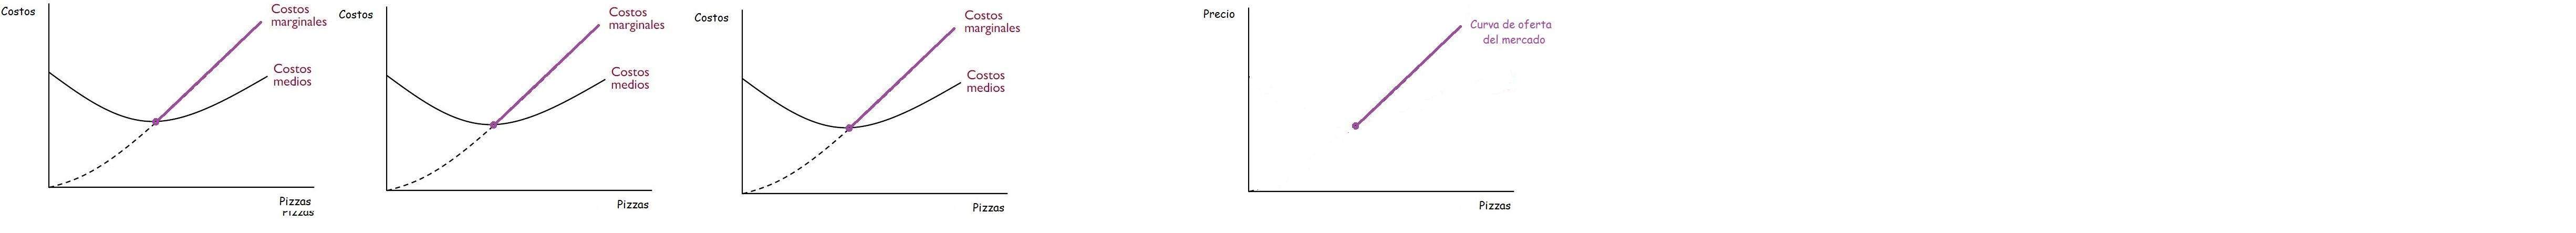
\includegraphics[scale=0.15]{Figures/Tema_06.29.jpg}
\end{frame}

\end{document}
